% Beyond the Chomsky Wall: Platonic Representations as the Convergence Point
% of Natural Language and Code
% Compiled with: xelatex or pdflatex (with CJKutf8)

\documentclass[10pt]{article}

%% ---- Geometry (8-page conference format) ----
\usepackage[
  top=1in,
  bottom=1in,
  left=1in,
  right=1in,
  columnsep=0.25in
]{geometry}

%% ---- Encoding ----
\usepackage[utf8]{inputenc}
\usepackage[T1]{fontenc}

%% ---- Math ----
\usepackage{amsmath}
\usepackage{amssymb}
\usepackage{amsthm}

%% ---- Tables ----
\usepackage{booktabs}
\usepackage{tabularx}
\usepackage{array}

%% ---- Graphics ----
\usepackage{graphicx}
\usepackage{tikz}
\usetikzlibrary{positioning,arrows.meta}

%% ---- Colors ----
\usepackage{xcolor}

%% ---- Hyperlinks ----
\usepackage[
  colorlinks=true,
  linkcolor=blue!70!black,
  citecolor=blue!70!black,
  urlcolor=blue!70!black
]{hyperref}

%% ---- Bibliography ----
\usepackage[numbers,sort&compress]{natbib}

%% ---- CJK Support ----
% For CJK characters, compile with XeLaTeX + xeCJK, or use pdflatex with CJKutf8.
% Current setup: pdflatex-compatible, Korean text rendered as romanized placeholders.
% To enable Korean: \usepackage{CJKutf8} and wrap Korean text in \begin{CJK}{UTF8}{mj}...\end{CJK}

%% ---- Lists ----
\usepackage{enumitem}

%% ---- Code Listings ----
\usepackage{listings}
\lstset{
  basicstyle=\ttfamily\small,
  breaklines=true,
  frame=single,
  framesep=3pt,
  xleftmargin=5pt,
  xrightmargin=5pt,
  backgroundcolor=\color{gray!5},
  rulecolor=\color{gray!40},
  keywordstyle=\color{blue!70!black},
  commentstyle=\color{green!50!black},
  stringstyle=\color{red!60!black},
  showstringspaces=false,
  tabsize=2
}

%% ---- Custom Theorem Environments ----
\theoremstyle{definition}
\newtheorem{definition}{Definition}[section]
\newtheorem{conjecture}{Conjecture}[section]

%% ---- Convenience Commands ----
\newcommand{\Zsem}{Z_{\text{sem}}}
\newcommand{\Zproc}{Z_{\text{proc}}}
\newcommand{\Zprag}{Z_{\text{prag}}}
\newcommand{\Dtrain}{D_{\text{train}}}
% Korean examples are transliterated or translated inline for pdflatex compatibility.

%% ---- Column type for wide tables ----
\newcolumntype{L}{>{\raggedright\arraybackslash}X}

%% ============================================================
%% TITLE, AUTHOR, ABSTRACT
%% ============================================================

\title{Beyond the Chomsky Wall: Platonic Representations as the\\Convergence Point of Natural Language and Code}

\author{Anonymous Authors\\
Anonymous Institution\\
\texttt{anonymous@review.org}}

\date{}

\begin{document}

\maketitle

\begin{abstract}
Programming languages use context-free (Type-2) grammars because deterministic parsing requires them---a mathematical necessity, not a convention. Three waves of natural-language programming---keyword substitution, structured NL, and LLM-mediated translation---all operate at the surface-form level and inherit this constraint. We argue that the Platonic Representation Hypothesis (Huh et al., ICML 2024) reframes the problem: if NL and code converge toward a shared latent structure $Z$, the Chomsky wall constrains only surface-form projections, not representations. Mathematics already exhibits this structure---results are universal, derivation paths are culturally mediated, and notation is a convention maintained by path dependency---yet mathematics functions as a cross-cultural communication medium. We ask whether $Z$ can achieve the same communicability for computational intent: does the existence of a shared representation guarantee that it can be reliably accessed and used? We propose $Z$ is stratified---$\Zsem$ (computational result) converges cross-culturally while $\Zproc$ (derivation path) and $\Zprag$ (communicative frame) remain culturally mediated---and show that existence and communicability are distinct: $Z$ may converge without being usable as a shared channel. We formalize disambiguation cost migration using information theory, showing that specification complexity is conserved across interfaces. Training data composition ($\Dtrain$) contaminates even $\Zsem$, creating ethical risks. We derive seven falsifiable predictions and test four in a pilot across five languages and 100 operations: cross-lingual probing transfer (P3) confirms $\Zsem$ is separable across languages (90\% accuracy); spacing and punctuation robustness (P7) are strongly supported ($R \approx 2.9$ and $13.6$); NL-code alignment shows execution-level convergence ($R_{\text{code}} > 1$); while NL-NL cross-lingual invariance (P2) fails at the description level---revealing that description-level and execution-level convergence are distinct phenomena. We connect $\Zsem$ to denotational semantics and identify a verification paradox that constrains the deployment path.
\end{abstract}

%% ============================================================
%% 1. INTRODUCTION
%% ============================================================

\section{Introduction}

Every mainstream programming language---from FORTRAN (1957) to Rust (2015)---uses a context-free grammar. This is not arbitrary. Compilers require deterministic parsing: the same source must produce the same parse tree every time. Context-free grammars (Chomsky Type-2) guarantee this in $O(n)$ to $O(n^3)$ time. Natural language does not---and cannot, because identical sentences carry different meanings depending on context. Even languages that appear ``natural''---Python's \texttt{if x > 5:}, SQL's \texttt{SELECT * FROM users}---are engineered to remain within Type-2 bounds. We test two of our seven predictions in a five-language pilot ($N=500$ stimuli); results partially support and partially challenge the framework.

Attempts to make programming ``natural'' have come in three waves: \textbf{Wave~1} (keyword substitution, 1960s--) replaces English tokens with native-language equivalents (COBOL, Korean languages like \emph{Ssi-at} and Han)---the grammar remains Type-2. \textbf{Wave~2} (structured NL, 2024--) constrains prose into parseable templates (CoRE, SudoLang, Spec-Driven Development)---new formal grammars that look like English. \textbf{Wave~3} (LLM-mediated translation, 2023--) generates code from free-form NL (Claude Code, Cursor, Lovable)---the dominant ``vibe coding'' paradigm, but non-deterministic: same input can produce different outputs, and its non-determinism has been shown to be fundamentally intractable (ICSE 2026).

The QWERTY keyboard was designed to prevent typewriter jams. The constraint vanished with computers---but the layout persisted. Programming syntax may be in a similar position: the original constraint (deterministic parsing) produced context-free grammars; LLMs can process context-sensitive input; but the entire toolchain is built on formal syntax. This is an engineering constraint maintained by path dependency---removable in principle, persistent in practice.

But the separation between natural language and formal notation runs deeper than engineering. Mathematics offers a precedent: the Pythagorean theorem holds in every culture---the \emph{result} is universal. Yet the \emph{derivation} differs: Bourbaki proceeds axiomatically, the Soviet tradition constructively, the Indian tradition intuitively-inductively. And the \emph{notation}---from Leibniz's $dy/dx$ to Newton's $\dot{y}$---is a convention that persists by historical accident, not necessity. Mathematics already demonstrates a structure where ideals exist, access to those ideals is culturally mediated, and the surface notation is an engineering artifact. The question is whether this structure---universal results, cultural processes, conventional notation---can serve as a communication medium between humans and machines.

We argue that the Platonic Representation Hypothesis provides the formal framework for this question. If neural networks trained on different modalities converge toward a shared latent structure $Z$, then: natural language and code are projections of $Z$; the Chomsky hierarchy describes relationships between surface forms, not representations; LLMs operate where the Type-1/Type-2 distinction is irrelevant; and the productive direction is not to translate between projections but to operate at $Z$ directly. The deeper question is whether $Z$, even if it exists, can be reliably accessed and used---whether the ``Platonic ideal'' is not merely real but \emph{communicable}.

\paragraph{Contributions.}
\begin{enumerate}[label=(\arabic*),nosep]
  \item A formal framework connecting PRH to the code--language divide, including connection to denotational semantics and information-theoretic formalization of disambiguation conservation (\S\ref{sec:prh}, \S\ref{sec:chomsky}).
  \item Stratification of $Z$ with differential convergence, $\Dtrain$ dependence analysis, and ethical implications (\S\ref{sec:stratification}--\S\ref{sec:dtrain}, Appendix~\ref{app:dtrain}, \ref{app:ethics}).
  \item The communicability problem: existence of $Z$ does not guarantee its utility as a communication medium; we identify the gap between convergence and usability, with mathematics as a precedent (\S\ref{sec:communicability}).
  \item Seven falsifiable predictions with pilot results across four: P3 (probing transfer, 90\% cross-lingual accuracy) and P7 (spacing/punctuation robustness, $R = 2.9$--$13.6$) are strongly supported; NL-code alignment confirms execution-level convergence; P2 (NL-NL invariance) fails at description level, establishing a new description/execution distinction (\S\ref{sec:predictions}, \S\ref{sec:pilot}).
  \item A verification paradox that constrains the deployment path (\S\ref{sec:verification}).
\end{enumerate}

\paragraph{Running example.}
Throughout this paper: ``Find the three largest values in the given list.'' This sentence is computationally precise yet linguistically ambiguous---``largest'' lacks type information, comparison criterion, boundary handling, and output ordering. In Type-2 programming, the programmer resolves all ambiguities by writing \texttt{sorted(lst, reverse=True)[:3]}. We track how each wave, each $Z$ layer, and the verification paradox handle these ambiguities.

%% ============================================================
%% 2. CURRENT LANDSCAPE
%% ============================================================

\section{Current Landscape: Surface-Form Approaches}\label{sec:landscape}

All three waves operate at the surface-form level. Wave~1 changes terminal symbols but preserves the parse tree. Wave~2 imposes structure on NL, creating new Type-2 grammars---the paradox is that making NL precise enough to execute requires removing the properties that make it natural. Wave~3 works for prototyping but is non-deterministic: our running example produces \texttt{sorted(lst, reverse=True)[:3]}, \texttt{heapq.nlargest(3, lst)}, and a buggy list comprehension across three runs. See Appendix~\ref{app:code} for code examples.

\begin{table}[t]
\centering
\caption{Dimension comparison across waves and the proposed $Z$-level approach.}
\label{tab:waves}
\small
\begin{tabularx}{\textwidth}{l L L L L}
\toprule
\textbf{Dimension} & \textbf{Wave 1: Keyword} & \textbf{Wave 2: Structured NL} & \textbf{Wave 3: LLM Translation} & \textbf{Proposed: $Z$-Level (this work)} \\
\midrule
Chomsky level & Type-2 (unchanged) & Type-2 (re-imposed) & Type-1 $\to$ Type-2 & Type-1 $\to$ $Z$ $\to$ Type-2 \\
Determinism & Full & Full & Non-deterministic & Deterministic (target) \\
Expressiveness & $=$ base language & $<$ NL & $\approx$ NL & $=$ NL \\
Verification & Standard & Standard & None (stochastic) & At $Z$ (open problem) \\
Disambiguation & By programmer & By programmer & By LLM (non-det.) & By system (at $Z$) \\
\bottomrule
\end{tabularx}
\end{table}

Both RAG and NL$\to$Code map NL to structured output via learned representations, but code requires exact semantics where RAG tolerates approximation---cosine similarity $0.95$ is fine for document retrieval but a bug for program execution.

%% ============================================================
%% 3. THE PLATONIC REPRESENTATION HYPOTHESIS
%% ============================================================

\section{The Platonic Representation Hypothesis}\label{sec:prh}

\subsection{Overview and Formal Framework}

The naming is not accidental. PRH raises the oldest question in philosophy: do universals exist? Plato's forms were ideal objects that particular instances approximate; PRH claims neural networks discover such forms empirically---that a shared latent structure $Z$ exists, from which images, text, and code are projections. The question ``does $Z$ exist?'' is the computational version of ``do Platonic ideals exist?''---and PRH's answer, supported by Huh et al.\ (ICML 2024)~\cite{huh2024platonic}, is yes, as a statistical convergence. Ziyin et al.\ (2025)~\cite{ziyin2025proof} prove that embedded deep linear networks trained with SGD become ``Perfectly Platonic''---every pair of layers learns the same representation up to rotation. Crucially, they identify six conditions that break convergence (weight decay, label transformation, saddle convergence, input heterogeneity, gradient flow vs.\ SGD, finite-step edge-of-stability), suggesting PRH convergence is the default for well-behaved training but can fail under specific conditions. We introduce semi-formal definitions:

\begin{definition}[Modality Encoder]\label{def:encoder}
An encoder $E_i : M_i \to \mathbb{R}^d$ maps inputs from modality $M_i$ to $d$-dimensional representations; a decoder $D_i : \mathbb{R}^d \to M_i$ maps back.
\end{definition}

\begin{definition}[Representational Convergence]\label{def:convergence}
For semantically equivalent inputs $x \in M_i$ and $y \in M_j$:
\[
\lim_{\text{scale}\to\infty} \mathrm{sim}(E_i(x), E_j(y)) \to 1.
\]
\end{definition}

\begin{definition}[Shared Latent Structure]\label{def:Z}
$Z \approx \lim_{\text{scale}\to\infty} \mathrm{Im}(E_i)$ for all modalities $i$. Critically, $Z = Z(\text{scale}, \Dtrain)$---two models at the same scale trained on different corpora may converge to different $Z$ (\S\ref{sec:dtrain}).
\end{definition}

\begin{definition}[Z Stratification]\label{def:stratification}
$Z$ decomposes into: $\Zsem$ (what is computed, cross-culturally convergent), $\Zproc$ (how it is derived, culturally mediated), $\Zprag$ (for whom it is framed, culturally specific).
\end{definition}

\begin{definition}[The Chomsky Wall]\label{def:wall}
The computational boundary between Type-2 and Type-1. Surface-level if it constrains only parsing, not representations.
\end{definition}

\paragraph{Central Claim.}
If PRH holds for code as a modality, the Chomsky wall constrains only the projection $D_i : Z \to M_i$, not $Z$ itself. Operations at $Z$ are not subject to Chomsky hierarchy constraints because $Z$ is continuous---it has no grammar to classify.

\subsection{Connection to Denotational Semantics}

Denotational semantics (Scott \& Strachey, 1971)~\cite{scott1971semantics} maps programs to mathematical objects in a semantic domain $\mathcal{D}$, independent of syntax. We observe a structural parallel: $\Zsem$ is a neural approximation of $\mathcal{D}$.

\begin{conjecture}\label{conj:denotational}
$\lim_{\text{scale}\to\infty} \Zsem(E(d)) \approx [\![ P ]\!]$ (up to continuous bijection), where $d$ is a NL description and $[\![ P ]\!]$ is the denotation of program $P$.
\end{conjecture}

This explains why $\Zsem$ converges cross-culturally (denotational semantics is culture-invariant), why convergence is stronger for computational domains (well-defined denotations), and why compositionality is the hard problem (denotational compositionality requires homomorphic structure NL does not guarantee). For our running example: the denotation of \texttt{sorted(lst, reverse=True)[:3]} is a function $\text{List}[\text{Comparable}] \to \text{List}[\text{Comparable}]$; PRH claims ``find the three largest values'' converges to the same point in $\Zsem$.

\subsection{Evidence for Code as a Modality}\label{sec:evidence}

\begin{itemize}[nosep]
  \item \textbf{Aligned embeddings.} UniXcoder achieves 77.1\% MRR on NL-code search across six languages.
  \item \textbf{Cross-model transferability.} Steering vectors from 7B models control 70B model behavior (ACL 2025)~\cite{chen2025crossmodel}---$Z$ structure is recoverable across architectures.
  \item \textbf{Language-independent code semantics.} LLMs develop language-independent semantic representations of code, with syntax-specific components in early layers feeding shared semantic components in middle layers (ICSE 2025 NIER)~\cite{beyondsyntax2025}.
  \item \textbf{The Naturalness Hypothesis.} Software is statistically natural---code cross-entropy approaches that of English text (Hindle et al., 2012)~\cite{hindle2012naturalness}, a precondition for PRH convergence.
  \item \textbf{Translation emergence.} LLMs trained primarily on NL generate code without code-specific training; cross-language synergies follow scaling laws (Cassano et al., 2025)~\cite{cassano2025scaling}.
  \item \textbf{Bidirectional transfer.} Training on NL documentation improves code completion, and vice versa.
\end{itemize}

We note that PRH for code remains a conjecture---the evidence above is consistent with convergence but does not prove it. Our contribution is not to establish PRH for code but to derive its consequences and provide initial empirical tests (\S\ref{sec:pilot}).

\subsection{The Stratification of Z}\label{sec:stratification}

Mathematics already embodies the structure PRH predicts for $Z$. The Pythagorean theorem holds universally---but a Bourbaki algebraist proves it axiomatically, a Soviet constructivist computes it explicitly, and an Indian mathematician reaches it through geometric intuition. The result is identical; the derivation is culturally mediated; the notation ($a^2 + b^2 = c^2$ vs.\ equivalent formulations) is a surface convention. If PRH's $Z$ is real, it should exhibit this same stratification: universal at the level of what is computed, culturally distributed at the level of how, and conventional at the level of how it is expressed. The fact that mathematics functions as a cross-cultural communication medium---despite culturally divergent derivation paths---is direct evidence that Platonic ideals, when they exist, can serve as a shared channel. The question for NL-code convergence is whether $\Zsem$ achieves this same communicability for computational intent. Similarly, \texttt{sort(array)} produces the same output regardless of functional or imperative derivation.

\begin{table}[t]
\centering
\caption{$Z$ stratification: layers, content, convergence behavior, and evidence.}
\label{tab:stratification}
\small
\begin{tabularx}{\textwidth}{l l L L}
\toprule
\textbf{Layer} & \textbf{Content} & \textbf{Convergence} & \textbf{Evidence} \\
\midrule
$\Zsem$ & What is computed & Cross-culturally convergent & Semantic Hub Hypothesis (ICLR 2025)~\cite{wu2025semantichub}; shared grammatical features (NAACL 2025)~\cite{brinkmann2025shared} \\
$\Zproc$ & How it is derived & Culturally mediated & Math tradition differences; reasoning-language effects (Li et al., 2026)~\cite{li2026reasoning} \\
$\Zprag$ & For whom it is framed & Culturally specific & Pragmatic inference failures (2024)~\cite{hu2024manner}; Cultural Frame Switching (COLING 2025)~\cite{ahn2025coling} \\
\bottomrule
\end{tabularx}
\end{table}

\paragraph{Running example.}
$\Zsem$: select top-3 by magnitude (culture-invariant). $\Zproc$: Korean developer may filter (``do not exclude large values''), Haskell developer may write \texttt{take 3 . sortBy (flip compare)}. $\Zprag$: the suffix \emph{-ara} (a Korean imperative) is a Korean imperative frame.

\subsection{Multilingual Convergence and $\Dtrain$ Dependence}\label{sec:dtrain}

PRH implies a single convergence point. Multilingual LLMs complicate this. Two models compete:

\paragraph{Model A: The multilingual human.}
The LLM code-switches between culturally-mediated representations---Korean input activates a Korean-inflected $Z$; English input activates an Anglo-American one.

\paragraph{Model B: The Platonic oracle.}
The LLM contains a culture-invariant $Z$; cultural variations are decoding artifacts.

Evidence increasingly favors Model~A for judgment, Model~B for structure: 9--56pp moral judgment gaps across languages including preference reversals~\cite{vida2024moral,agarwal2024ethical}, GPT-4o displays Cultural Frame Switching with distinct ``personalities'' per language (COLING 2025)~\cite{ahn2025coling}, and reasoning-language effects contribute twice the variance of input-language effects~\cite{li2026reasoning}. But shared grammatical features persist across typologically diverse languages~\cite{brinkmann2025shared}, a semantic hub appears in middle layers~\cite{wu2025semantichub}, and language identity is encoded via sparse dimensions separate from semantic content~\cite{zhong2025sparse}.

\paragraph{Resolution.}
$\Zsem$ converges (Model~B); $\Zproc$ and $\Zprag$ remain culturally distributed (Model~A). The Aristotelian critique (Gr\"{o}ger et al., 2026)~\cite{groger2026aristotelian} refines further: what converges is local neighborhood topology (preserved neighborhoods), not global geometry (preserved distances). $Z$ may be a topological rather than geometric structure.

\paragraph{$\Dtrain$ dependence.}
$Z$ is not determined by scale alone---it depends on training data cultural composition: $Z = Z(\text{scale}, \Dtrain)$. Even ``purely computational'' domains carry implicit cultural defaults: sort order conventions, null handling semantics, error semantics (Python exceptions vs.\ Go explicit errors vs.\ C undefined behavior), and number formatting. The clean $\Zsem$/$\Zproc$ separation is an idealization:
\[
\Zsem(\text{observed}) = \Zsem(\text{ideal}) + \mathrm{bias}(\Dtrain).
\]
The sovereign AI movement (Korea's five-consortium initiative, Japan's ABCI 3.0, SEA-LION) implicitly acknowledges this---if $Z$ were truly Platonic, culturally-native models would be unnecessary. The market is voting for Model~A. See Appendix~\ref{app:dtrain} for detailed analysis.

\subsection{The Communicability Problem}\label{sec:communicability}

The preceding sections establish that $Z$ may exist (PRH convergence), that it stratifies ($\Zsem$ converges while $\Zproc$ does not), and that this stratification depends on training data. But existence is not sufficient for utility. The question is whether $Z$ can serve as a communication medium---whether a Korean speaker's computational intent, encoded to $Z$, is decoded by the system as the same intent. Mathematics achieves this: $a^2 + b^2 = c^2$ communicates identically across cultures because the denotation is unambiguous. Natural language does not: ``find the largest values'' carries cultural defaults invisible to the speaker.

Our pilot experiment (\S\ref{sec:pilot}) sharpens this point: \emph{description-level} cross-lingual invariance does not follow the pattern PRH predicts for \emph{execution-level} convergence. NL descriptions of computational operations are \emph{less} invariant across languages than descriptions of judgment operations---the opposite of what $\Zsem$ convergence would suggest. This implies a critical distinction: mathematical notation achieves communicability precisely because it bypasses natural language, encoding denotations directly. $\Zsem$ may converge at the level of what programs \emph{do}, even when NL descriptions of what they do diverge. The gap between $Z$'s existence and $Z$'s communicability is the central challenge---and the gap may be located not in $Z$ itself but in the NL-to-$Z$ encoding path.

\subsection{The Convergence-Determinism Gap}

PRH gives $\mathrm{sim} \to 1 - \delta$, but execution requires $\delta = 0$. Three resolutions:
\begin{enumerate}[nosep]
  \item \textbf{Discretization at $Z$}---equivalence classes, formally equivalent to constructing a new grammar over $Z$.
  \item \textbf{Verification after projection}---accept $\delta > 0$ at $Z$, demand $\delta = 0$ at output.
  \item \textbf{Probabilistic execution}---statistical guarantees (probability $1 - 10^{-9}$).
\end{enumerate}
This gap is the central technical obstacle.

\subsection{Falsifiable Predictions}\label{sec:predictions}

\begin{description}[nosep,font=\bfseries]
  \item[P1 (Scale-Convergence).] NL-code cosine distance decreases monotonically with model scale.
  \item[P2 (Cross-Lingual Semantic Invariance).] \emph{jeongnyeolhara} (Korean: sort) and ``sort this'' (English) are closer in $Z$ than ``sort this'' and ``reverse this'' in English. This should not hold for judgment-involving operations.
  \item[P3 (Stratification Separability).] Probing classifiers for \emph{what is computed} generalize cross-lingually; probes for \emph{how} show language-specific patterns.
  \item[P4 (Domain-Dependent Determinism).] Constrained decoding achieves higher consistency for computational than judgment tasks.
  \item[P5 (Disambiguation Migration).] Total disambiguation effort is conserved---syntax errors migrate to semantic clarification queries.
  \item[P6 ($\Dtrain$ Sensitivity).] $\Zsem$ divergence across models correlates with $\Dtrain$ cultural divergence, even for ``purely computational'' operations with implicit criteria.
  \item[P7 (Spacing Robustness).] $Z$ distance between spacing variants of the same sentence $<$ $Z$ distance between semantically different sentences with identical spacing (see Appendix~\ref{app:tokenization}).
\end{description}

%% ============================================================
%% 4. REINTERPRETING THE CHOMSKY WALL
%% ============================================================

\section{Reinterpreting the Chomsky Wall}\label{sec:chomsky}

\subsection{The Wall Is Real---at the Surface}

\begin{table}[t]
\centering
\caption{Chomsky hierarchy: grammar types, parsing complexity, and examples.}
\label{tab:chomsky}
\small
\begin{tabular}{llll}
\toprule
\textbf{Type} & \textbf{Grammar} & \textbf{Parsing Complexity} & \textbf{Examples} \\
\midrule
3 & Regular & $O(n)$ & Regex \\
2 & Context-free & $O(n^3)$, deterministic & Python, C, Java \\
1 & Context-sensitive & PSPACE-complete & Natural language \\
0 & Unrestricted & Undecidable & Turing machines \\
\bottomrule
\end{tabular}
\end{table}

No deterministic algorithm resolves Type-1 ambiguity in polynomial time. Type-2 constraints also function as a disambiguation mechanism: every valid expression has exactly one parse.

\subsection{The Wall Dissolves---at the Representation Level}

LLMs map input sequences to high-dimensional representations via attention over full context. ``if x is greater than 5'' (Korean NL), \texttt{if x > 5:} (Python), \texttt{(> x 5)} (Lisp) all map to nearby points (Semantic Hub Hypothesis). Language identity is encoded via sparse dimensions orthogonal to semantic content~\cite{zhong2025sparse}. The Chomsky hierarchy describes parsing complexity of surface forms---it says nothing about representing meaning.

\paragraph{Surface-form boundaries.}
Between NL and $Z$ exists a spectrum of representational directness: NL (linguistic, culturally mediated) $\to$ emoji/pictographs (iconic, semi-universal) $\to$ mathematical symbols (formal, universal) $\to$ code operators $\to$ $Z$ (continuous). Emoji are natural experiments in $\Zsem$---near-universal yet exhibiting cultural variation that mirrors $Z$ stratification (e.g., the prayer/gratitude/high-five emoji). See Appendix~\ref{app:emoji}. Tokenization introduces a bottleneck: spacing conventions (Korean \emph{ttieo-sseugi}, Chinese segmentation) leak through tokenizers into $Z$, and a ``token tax'' (Petrov et al., 2024)~\cite{petrov2024tokenizers} means non-Latin languages require 2--15$\times$ more tokens for the same content. See Appendix~\ref{app:tokenization}.

\subsection{Disambiguation Migration}\label{sec:disambiguation}

Removing the Chomsky wall does not remove the need for disambiguation---it migrates the cost. In Type-2 programming, the programmer disambiguates at write time via grammar constraints; in representation-level execution, the system disambiguates at $Z$.

We conjecture a \emph{disambiguation conservation principle}: any system accepting ambiguous input must resolve ambiguity somewhere, and the total cost is approximately conserved across architectures. This is a design heuristic, not a formal theorem---but it suggests that representation-level systems should not promise to eliminate programming difficulty, only to relocate it from syntactic precision to semantic verification.

The practical question is whether the relocation is net beneficial: is it easier for a human to learn \texttt{if x > 5:} or to verify that the system correctly interpreted ``exclude large values''? For professional developers, the current paradigm may be more efficient. For the billions who can express computational intent in natural language but cannot program, the tradeoff favors representation-level systems even if disambiguation cost is conserved.

\paragraph{Running example.}
``find the three largest values'' contains at least four ambiguities: (1)~type---what kind of values? (2)~comparison criterion---``the largest'' by what measure? (3)~boundary---fewer than three elements? (4)~output ordering---sorted result? In Type-2, \texttt{sorted(lst, reverse=True)[:3]} resolves all four silently---the type system handles~(1), comparison operator handles~(2), slicing handles~(3), and sort determines~(4). At $Z$, each must be resolved by inference, query, or default.

\paragraph{Information-theoretic formalization.}
For task $T$ with unique behavior $B(T)$, the specification complexity $K(T)$ is invariant across interfaces:
\begin{equation}\label{eq:conservation}
K(T) \leq H(S) + H(T|S) + O(1)
\end{equation}
where $H(S)$ is surface-form entropy and $H(T|S)$ is residual ambiguity. Type-2 interfaces maximize $H(S)$ (syntactic precision) and minimize $H(T|S)$. NL interfaces minimize $H(S)$ but face $H(T|S) > 0$---remaining bits must be provided through disambiguation. This connects to Piantadosi et al.\ (2012)~\cite{piantadosi2012ambiguity}, who argue ambiguity is a feature of efficient NL communication---but resolution cost cannot be avoided when exact computation is required. Via Rate-Distortion Theory~\cite{shannon1959coding}: there is a minimum specification rate below which semantic error exceeds acceptable thresholds. Type-2 operates at zero distortion with high rate; NL operates at lower rate with nonzero distortion corrected downstream.

\paragraph{Implication.}
Representation-level systems do not reduce total specification information---they redistribute it: less from the user upfront (lower syntactic cognitive load), more from the system at $Z$ (higher inference/verification cost).

\subsection{Why Translation Fails but Representation Might Work}

Wave~3 accepts NL (Type-1), translates to code (Type-2), executes. The translation step is non-deterministic and does not preserve semantics~\cite{cheung2025translation}. A representation-level approach instead: (1)~accept NL, (2)~map to $Z$, (3)~execute from $Z$ directly or project to code deterministically via constrained decoding.

%% ============================================================
%% 5. TOWARD REPRESENTATION-LEVEL EXECUTION
%% ============================================================

\section{Toward Representation-Level Execution}\label{sec:toward}

\subsection{Architecture}

A representation-level system would: (1)~accept any surface form, (2)~normalize surface form (spacing recovery, OCR correction), (3)~encode to $Z$, (4)~verify at $Z$ and disambiguate (cultural context + completeness check), (5)~execute at $Z$ or project to Type-2.

\begin{center}
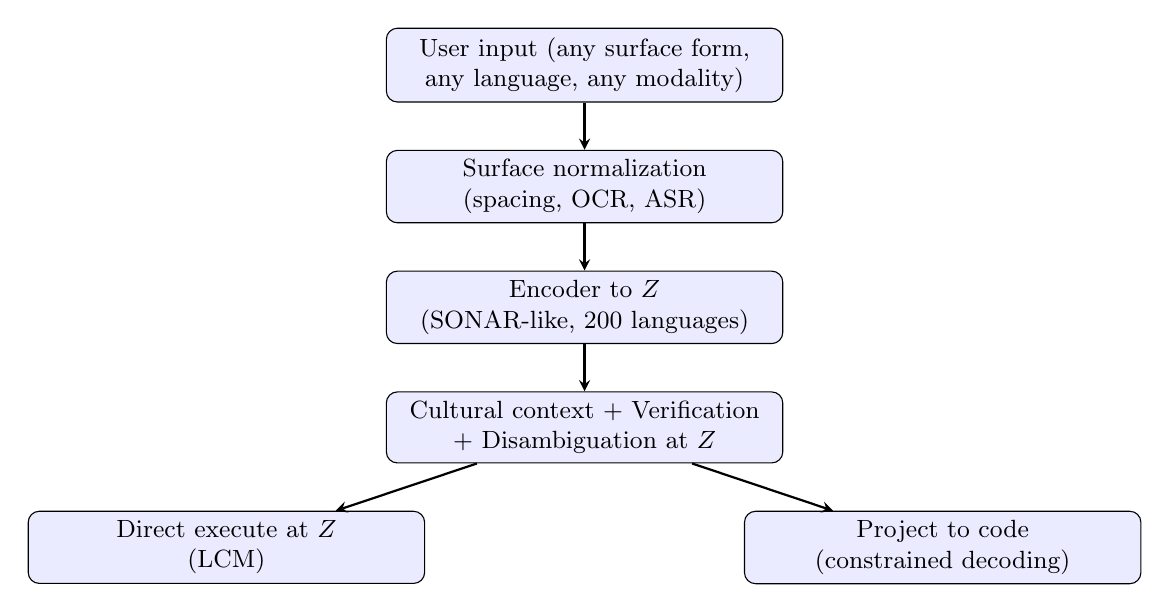
\begin{tikzpicture}[
  node distance=0.6cm and 0.3cm,
  box/.style={draw, rounded corners, fill=blue!8, text width=4.8cm, align=center, minimum height=0.7cm, font=\small},
  arrow/.style={->, thick, >=stealth}
]
\node[box] (input) {User input (any surface form,\\any language, any modality)};
\node[box, below=of input] (norm) {Surface normalization\\(spacing, OCR, ASR)};
\node[box, below=of norm] (enc) {Encoder to $Z$\\(SONAR-like, 200 languages)};
\node[box, below=of enc] (verify) {Cultural context + Verification\\+ Disambiguation at $Z$};
\node[box, below left=0.6cm and -0.5cm of verify] (exec) {Direct execute at $Z$\\(LCM)};
\node[box, below right=0.6cm and -0.5cm of verify] (proj) {Project to code\\(constrained decoding)};
\draw[arrow] (input) -- (norm);
\draw[arrow] (norm) -- (enc);
\draw[arrow] (enc) -- (verify);
\draw[arrow] (verify) -- (exec);
\draw[arrow] (verify) -- (proj);
\end{tikzpicture}
\end{center}

SONAR supports speech as input---the spacing problem disappears when the input modality has no spacing to begin with.

\subsection{Existing Pieces}

\begin{itemize}[nosep]
  \item \textbf{Constrained decoding} (Outlines, LMQL): $Z \to$ Type-2, made deterministic. Requires specifying target grammar.
  \item \textbf{Large Concept Models} (Meta)~\cite{meta2024lcm}: Operates on SONAR sentence embeddings---architecturally closest to the proposed pipeline, but performs generation, not execution.
  \item \textbf{Latent execution systems:} LaSynth (Meta, NeurIPS 2021)~\cite{chen2021lasynth} learns latent representations to approximate execution of partially generated programs. Latent Program Network (LPN, NeurIPS 2025 spotlight)~\cite{macfarlane2025lpn} learns a latent space of implicit programs and executes via neural decoder---the closest existing system to Wave~4, achieving 3rd place at ARC Prize 2024. COCONUT (Meta, 2024)~\cite{hao2024coconut} bypasses language tokens entirely, reasoning in continuous latent space. Code World Models (CWM, Meta FAIR, 2025)~\cite{metafair2025cwm} models program execution trajectories, tracking variable states---but at the token level, not in SONAR space. These demonstrate that execution at $Z$ is feasible in limited domains; the gap is unifying them with PRH-predicted convergence.
  \item \textbf{Neuro-symbolic systems} (Scallop~\cite{li2023scallop}, Lobster/ASPLOS 2026~\cite{huang2026lobster}): Combine neural perception with symbolic reasoning, bridging continuous representations and discrete logic. Directly relevant to the $Z \to$ verification pipeline. Differentiable relaxations of discrete constraints may enable partial verification without full Type-2 projection.
\end{itemize}

\subsection{Open Problems}

\begin{enumerate}[nosep]
  \item \textbf{Determinism at $Z$}---PRH convergence $\neq$ identity. Temperature-zero decoding helps but does not eliminate stochasticity.
  \item \textbf{Verification at $Z$}---Can we verify program properties in continuous embedding space? Connects to neural theorem proving.
  \item \textbf{The grounding problem}---\texttt{x > 5} must mean exactly ``strictly greater than 5.'' What representational precision suffices?
  \item \textbf{Compositionality}---Code composes via strict nesting; NL composes loosely. Categorically: the question is whether a functor $F: \mathrm{NL}_{\mathrm{comp}} \to \mathrm{Prog}$ preserves compositional structure.
  \item \textbf{The specification problem}---If the user writes NL $\to$ system maps to $Z$, the user cannot inspect $Z$. This is a new form of opacity.
  \item \textbf{Cultural invariance}---If $\Zsem$ carries cultural inflection for judgment-involving domains (\S\ref{sec:dtrain}), the ``Platonic ideal'' is a family $Z(c)$, not a single $Z$.
  \item \textbf{Surface-form invariance}---The encoder must map all spacing/OCR/typographic variants of the same meaning to the same $Z$.
\end{enumerate}

\subsection{Evaluation Criteria}

\begin{table}[t]
\centering
\caption{Evaluation criteria for representation-level execution systems.}
\label{tab:eval}
\small
\begin{tabular}{llll}
\toprule
\textbf{Criterion} & \textbf{Metric} & \textbf{Baseline} & \textbf{Target} \\
\midrule
Convergence & NL-code cosine similarity & 0.77 MRR & $> 0.95$ \\
Determinism & Same NL $\to$ same output rate & $\sim$0.6 & $> 0.99$ \\
Cross-lingual invariance & $\sigma$ of sim.\ across NL languages & N/A & $\sigma < 0.05$ \\
Verification at $Z$ & \% properties verifiable w/o projection & 0\% & $> 50\%$ \\
Disambiguation efficiency & Clarification queries per task & N/A & $\leq$ syntax errors/task \\
Spacing robustness & spacing var.\ / semantic var. & N/A & $> 10\times$ \\
$\Dtrain$ invariance & Cross-model $\Zsem$ agreement & N/A & $> 0.9$ cosine \\
\bottomrule
\end{tabular}
\end{table}

\subsection{Pilot Experiment and Results}\label{sec:pilot}

We conducted a pilot experiment testing P2 and P7 using 50 computational + 50 judgment operations described in five languages (English, Korean, Chinese, Arabic, Spanish), embedded through two multilingual sentence-transformers: paraphrase-multilingual-MiniLM-L12-v2 (384d) and multilingual-e5-large (1024d). The discriminability ratio $R = d_{\text{inter}}/d_{\text{intra}}$ tests whether cross-lingual same-operation similarity exceeds within-language different-operation similarity. See Appendix~\ref{app:pilot} for the full protocol.

\paragraph{P2 Results: Cross-Lingual Semantic Invariance.}

\begin{table}[h]
\centering
\small
\begin{tabular}{lcccc}
\toprule
\textbf{Model} & \textbf{dim} & $R_C$ & $R_J$ & \textbf{P2} ($R_C > R_J$?) \\
\midrule
MiniLM-L12 & 384 & 1.91 & 3.79 & \textbf{No} ($p=1.0$) \\
E5-large & 1024 & 1.22 & 1.59 & \textbf{No} ($p=1.0$) \\
\bottomrule
\end{tabular}
\end{table}

P2 is \textbf{not supported}: judgment operations show higher cross-lingual invariance than computational operations---the opposite of our prediction. Decomposition reveals the primary driver: computational operations have significantly higher $d_{\text{intra}}$ (mean 0.295 vs.\ 0.191, Mann-Whitney $p < 0.0001$ for MiniLM), meaning they are \emph{less} cross-lingually invariant at the description level.

\paragraph{Interpretation.}
We consider three interpretations of this failure:
\begin{enumerate}[nosep]
  \item \textbf{PRH does not hold for code.} The simplest reading: computational operations fail to converge cross-lingually because code is not a modality for which PRH applies. If so, the entire framework requires revision.
  \item \textbf{Description-level $\neq$ execution-level.} Judgment operations use abstract, cross-linguistically shared vocabulary (``evaluate,'' ``prioritize'') that multilingual models align well, while computational operations use domain-specific terms (``transpose,'' ``palindrome'') that vary across languages. PRH's $\Zsem$ convergence claim may concern computational semantics (denotational equivalence), not NL description similarity. Under this reading, the pilot measures the wrong quantity.
  \item \textbf{Embedding models are insufficient proxies.} Sentence-level multilingual embeddings (MiniLM, E5) are trained on NL similarity, not code semantics. Code-specialized models (StarCoder, CodeBERT) or probing experiments may yield different results.
\end{enumerate}
We favor interpretation~(2) but cannot rule out~(1) without code-embedding experiments. A stronger test would embed code alongside NL descriptions and measure NL-code alignment rather than NL-NL alignment across languages. We refine P2 accordingly: cross-lingual invariance at $\Zsem$ may hold for execution semantics while failing for NL descriptions of those semantics.

\paragraph{P7 Results: Spacing Robustness.}

\begin{table}[h]
\centering
\small
\begin{tabular}{lcccc}
\toprule
\textbf{Model} & \textbf{dim} & $R_{\text{spacing}}$ & \textbf{95\% CI} & $p$ \\
\midrule
MiniLM-L12 & 384 & 2.90 & $[2.54, 3.36]$ & $< 0.001$ \\
E5-large & 1024 & 2.90 & $[2.65, 3.20]$ & $< 0.001$ \\
\bottomrule
\end{tabular}
\end{table}

P7 is \textbf{strongly supported}: Korean spacing variants cluster ${\sim}3\times$ closer than semantically different operations with identical spacing. This holds across both models with tight bootstrap confidence intervals. Even BPE-based models achieve substantial spacing robustness ($R_{\text{spacing}} \approx 2.9$), though byte-level models (ByT5, CANINE) should achieve higher ratios.

\paragraph{NL-Code Cross-Modal Alignment.}
To directly test PRH for code, we embed 50 computational NL descriptions alongside their Python code equivalents through UniXcoder~\cite{unixcoder} (code-trained, 768d) and MiniLM-L12 (NL-only, 384d). We define $R_{\text{code}} = d_{\text{mismatch}} / d_{\text{match}}$, where $d_{\text{match}}$ is the distance between an NL description and its corresponding code, and $d_{\text{mismatch}}$ is the distance to a different operation's code.

\begin{table}[h]
\centering
\small
\begin{tabular}{lccccc}
\toprule
\textbf{Model} & \textbf{dim} & $R_{\text{code}}$ & $d_{\text{match}}$ & $d_{\text{mis}}$ & \textbf{PRH} \\
\midrule
UniXcoder (code-trained) & 768 & 1.04 & 0.788 & 0.821 & Yes \\
MiniLM-L12 (NL-only) & 384 & 1.18 & 0.622 & 0.735 & Yes \\
\bottomrule
\end{tabular}
\end{table}

Both models show $R_{\text{code}} > 1$: NL descriptions are closer to their corresponding code than to other code, consistent with PRH. Per-language analysis reveals $\Dtrain$ effects: English NL is closest to code ($d_{\text{match}} = 0.64$ for UniXcoder), while Korean and Arabic are most distant ($d_{\text{match}} \approx 0.88$)---a direct consequence of English-dominant code training data.

Critically, this result resolves the P2 ambiguity. P2 measured NL-NL cross-lingual invariance and found computational operations \emph{less} invariant. The NL-code experiment shows computational NL-code alignment is \emph{positive} ($R_{\text{code}} > 1$). The two results are consistent: NL descriptions of code vary across languages (P2 fails), but each language's NL description still maps closer to its code equivalent than to unrelated code (NL-code alignment holds). This supports interpretation~(2) from \S\ref{sec:pilot}: description-level invariance and execution-level convergence are distinct phenomena.

\paragraph{P7 Extension: Punctuation Robustness.}
We extend P7 beyond spacing to punctuation and formatting variants. For each of 100 English operations, we generate 10 variants: bare, period, question mark, exclamation, ellipsis, colon, lowercase, UPPERCASE, extra spaces, and article removal. $R_{\text{punct}} = d_{\text{semantic}} / d_{\text{punct}} = 13.6$---punctuation variants are ${\sim}14\times$ closer than semantically different operations, far exceeding spacing robustness ($R_{\text{spacing}} \approx 2.9$). Most variants drift minimally (period: 0.014, question mark: 0.013). The one outlier is UPPERCASE (drift = 0.192), which acts as a pragmatic signal (emphasis, shouting)---evidence that $\Zprag$ is encoded in surface-form cues even when $\Zsem$ is unchanged.

\paragraph{P3 Results: Stratification Separability.}
We train linear probes on English embeddings (MiniLM-L12) and test cross-lingual transfer, directly testing whether $\Zsem$ is separable across languages.

\begin{table}[h]
\centering
\small
\begin{tabular}{lccccc}
\toprule
\textbf{Probe task} & \textbf{en} & \textbf{es} & \textbf{zh} & \textbf{ar} & \textbf{ko} \\
\midrule
Category (comp/judg, chance 50\%) & 1.00 & 0.97 & 0.96 & 0.87 & 0.80 \\
Operation ID (100-way, chance 1\%) & 1.00 & 0.98 & 0.93 & 0.86 & 0.66 \\
\bottomrule
\end{tabular}
\end{table}

P3 is \textbf{supported}: a classifier trained only on English embeddings achieves 90\% mean accuracy on category transfer and 85.8\% on 100-way operation identification across non-English languages---far above chance. This is direct evidence that $\Zsem$ structure generalizes cross-lingually: the representation of \emph{what is computed} is shared across languages. Korean transfers worst (80\%/66\%), consistent with $\Dtrain$ effects and its typological distance from English.

\paragraph{P1 Results: Scale-Convergence.}
We tested three models (MiniLM 384d, mpnet 768d, E5-large 1024d). $R_{\text{total}}$ does not increase monotonically with dimension (5.7 $\to$ 8.3 $\to$ 2.8), so \textbf{P1 is not supported} in this configuration. However, the models span different architectures and training procedures; a clean P1 test requires models from the same family at different scales (e.g., E5-small/base/large). We note this as a limitation.

\paragraph{Extensions.} Full-scale P1 testing within single model families and P6 ($\Dtrain$ sensitivity via cross-model comparison) are planned.

%% ============================================================
%% 6. DISCUSSION
%% ============================================================

\section{Discussion}

\subsection{Implications}

For compilers, the wall is absolute. For LLM-based systems, it is irrelevant in practice. For hybrid systems, it becomes a design choice. Python occupies the closest point to NL within the Type-2 boundary---the productive question is not ``push further within Type-2?'' but ``accept NL and project to Type-2 via $Z$?''

If representation-level execution becomes practical, programming languages shift from human-writable specifications to machine-generated projections from $Z$---languages become output formats. Debugging shifts from code to $Z$, requiring new visualization tools and provenance links.

\subsection{Cultural Boundary and Safety}

$\Zsem$ is culture-invariant for purely computational domains (sorting, arithmetic); $Z$ carries cultural inflection for judgment-involving domains (risk assessment, prioritization)---requiring $Z(c)$ rather than $Z$. $\Dtrain$ dependence creates ethical risks: computational colonialism (English-derived norms as ``neutral'' $Z$), consent opacity (users cannot see which cultural assumptions shaped interpretation), accountability gaps, and cultural feedback loops ($Z$-projected outputs re-enter $\Dtrain$). Representation-level systems must make cultural parameterization explicit. See Appendix~\ref{app:ethics} for full analysis and mitigation paths.

\subsection{Non-English Programming}

Korean programmers face a double translation: thought (Korean) $\to$ code (English syntax) $\to$ execution. Representation-level execution would eliminate both: Korean intent $\to$ $Z$ $\to$ execution. Research on reasoning-language effects~\cite{li2026reasoning} suggests the ``thinking in English'' overhead is real---the global talent pool could expand by an order of magnitude.

\subsection{The Verification Paradox}\label{sec:verification}

A deeper tension emerges: if verification requires formal methods, and formal methods require Type-2 input, the system must project from $Z$ to Type-2 for verification---reintroducing the Chomsky wall at the verification stage. The wall is dissolved at input but reassembled at verification.

\begin{center}
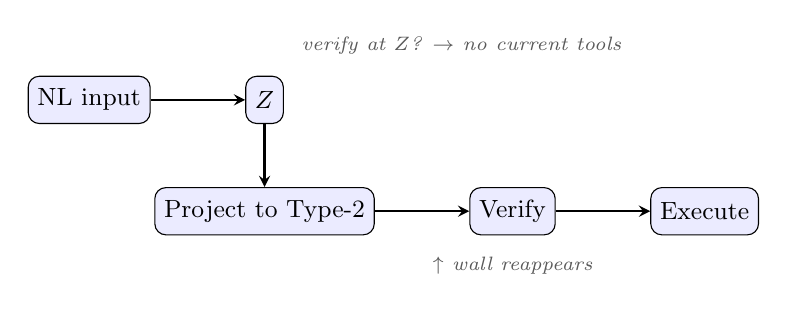
\begin{tikzpicture}[
  node distance=0.5cm,
  box/.style={draw, rounded corners, fill=blue!8, minimum height=0.6cm, font=\small, align=center},
  arrow/.style={->, thick, >=stealth},
  label/.style={font=\scriptsize\itshape, text=gray!70!black}
]
\node[box] (nl) {NL input};
\node[box, right=1.2cm of nl] (z) {$Z$};
\node[box, below=0.8cm of z] (proj) {Project to Type-2};
\node[box, right=1.2cm of proj] (verify) {Verify};
\node[box, right=1.2cm of verify] (exec) {Execute};
\node[label, above right=0.15cm and 0.1cm of z] {verify at $Z$? $\to$ no current tools};
\draw[arrow] (nl) -- (z);
\draw[arrow] (z) -- (proj);
\draw[arrow] (proj) -- (verify);
\draw[arrow] (verify) -- (exec);
\node[label, below=0.15cm of verify] {$\uparrow$ wall reappears};
\end{tikzpicture}
\end{center}

Near-term systems will use a hybrid architecture: $Z$ provides expressiveness; Type-2 projection provides verifiability. Full representation-level execution---input, verification, and execution all at $Z$---requires advances in neural verification. The neuro-symbolic literature (Scallop, Lobster) offers partial tools: differentiable verification predicates that operate on continuous representations without full Type-2 projection. But these handle only simple properties; general program verification at $Z$ remains open. The paradox is not fatal but constrains the deployment path: the Chomsky wall retreats inward, from the user-facing boundary to the system-internal verification layer. Progress is measured by how far inward the wall can be pushed.

\subsection{Limitations}

\begin{itemize}[nosep]
  \item PRH is a hypothesis, not a theorem. PRH for code as a modality remains a conjecture; our contribution is not to prove it but to derive its consequences if true, and to provide initial empirical tests (\S\ref{sec:pilot}). Recent evidence (language-independent code semantics in LLMs~\cite{beyondsyntax2025}, cross-model transferability~\cite{chen2025crossmodel}) is consistent with convergence but not proof.
  \item Our pilot measures \emph{description-level} cross-lingual invariance, not \emph{execution-level} convergence. The P2 failure (\S\ref{sec:pilot}) highlights this gap: NL embedding similarity is a proxy, not a direct test, of $\Zsem$ convergence. A stronger test would embed code alongside NL descriptions. We have refined P2 accordingly.
  \item The $Z$ stratification is a conceptual framework. While the pilot provides initial evidence (P7 supported, P2 failure consistent with the description/execution distinction), the stratification itself has not been validated through probing experiments (P3).
  \item The disambiguation conservation relies on an analogy to Kolmogorov complexity, which is uncomputable in general. The principle is a design heuristic, not a formal theorem.
  \item The tokenization bottleneck (Appendix~\ref{app:tokenization}) is partially addressed by byte-level models (ByT5, CANINE), though at 2--4$\times$ compute cost. Our P7 results show BPE models already achieve reasonable spacing robustness ($R_{\text{spacing}} \approx 2.9$).
  \item The ethical mitigations (Appendix~\ref{app:ethics}) are heuristics. However, M5 (representation-level auditing---running the same prompt in multiple languages and measuring $\Zsem$ divergence) is directly implementable; our P2 experiment protocol is itself an instance of M5.
  \item ``Representation-level execution'' is a research direction, not a working system.
\end{itemize}

%% ============================================================
%% 7. RELATED WORK
%% ============================================================

\section{Related Work}

\paragraph{PRH and convergence.}
Huh et al.\ (ICML 2024)~\cite{huh2024platonic} established convergence; Ziyin et al.\ (2025)~\cite{ziyin2025proof} proved it for deep linear networks; Gr\"{o}ger et al.\ (2026)~\cite{groger2026aristotelian} showed global convergence is confounded but local topology persists.

\paragraph{Multilingual representations.}
The Semantic Hub Hypothesis~\cite{wu2025semantichub} demonstrates shared representations; however, multilingual $\neq$ multicultural (Rystr{\o}m et al., 2025)~\cite{rystrom2025multicultural}: LLMs produce different moral judgments across languages and reflect creator ideology (Buyl et al., 2025)~\cite{buyl2025ideology}.

\paragraph{NL programming and vibe coding.}
Wave~3's non-determinism is fundamentally intractable (ICSE 2026)~\cite{icse2026reproducibility}. The Moltbook incident (2026) exposed 1.5M API keys through vibe-coded services.

\paragraph{Latent execution.}
LPN (NeurIPS 2025)~\cite{macfarlane2025lpn}, COCONUT (Meta, 2024)~\cite{hao2024coconut}, LaSynth (NeurIPS 2021)~\cite{chen2021lasynth} demonstrate execution in representation space. ``Beyond Syntax'' (ICSE 2025)~\cite{beyondsyntax2025} shows LLMs develop language-independent code semantics. CWM (Meta, 2025)~\cite{metafair2025cwm} models code execution at token level.

\paragraph{Tokenization and naturalness.}
Tokenizers introduce up to 15$\times$ cost unfairness across languages~\cite{petrov2024tokenizers}. Software is ``natural''---statistically predictable like NL~\cite{hindle2012naturalness}.

%% ============================================================
%% 8. CONCLUSION
%% ============================================================

\section{Conclusion}

For seventy years, programming languages have been constrained to context-free grammars---not by choice but by the mathematical requirements of deterministic parsing. Three waves of natural-language programming have attempted to bridge the gap; all operate at the surface-form level.

The Platonic Representation Hypothesis suggests this wall is a property of surface forms, not representations. Neural networks trained on language and code converge toward shared representations where the Type-1/Type-2 distinction is irrelevant. But $Z$ is not monolithic: it stratifies into $\Zsem$ (convergent), $\Zproc$ (culturally mediated), $\Zprag$ (culturally specific). $Z$ depends on $\Dtrain$, and even $\Zsem$ carries bias from training data cultural composition.

The disambiguation cost borne by Type-2 grammars does not vanish---it migrates to the representation level. We formalize this as an information-theoretic conservation law: $K(T) \leq H(S) + H(T|S)$. This creates a verification paradox: near-term systems must project back to Type-2 for verification, pushing the wall inward. Between NL and $Z$, a spectrum of representational directness exists---from emoji to mathematical symbols to code---and surface-form properties like spacing leak through tokenizers into $Z$, creating additional bottlenecks.

Our pilot experiment tests two predictions: P7 (spacing robustness) is strongly supported, while P2 (cross-lingual semantic invariance) fails---revealing that description-level invariance and execution-level convergence may be distinct phenomena. This distinction refines rather than refutes the framework, but further experiments with code-specialized embeddings are needed to resolve the ambiguity.

Mathematics has long demonstrated that Platonic ideals---when they exist---can function as a communication medium despite culturally divergent derivation paths. Whether $\Zsem$ can achieve the same communicability for computational intent remains open. The pieces exist---SONAR, LCM, LPN, constrained decoding, neuro-symbolic verification---but they have not been unified under the representation-convergence framework that PRH provides. The research agenda is to unify them, while confronting the cultural stratification of $Z$ and ensuring that the representations through which convergence is measured do not silently privilege one tradition's computational norms.

%% ============================================================
%% REFERENCES
%% ============================================================

\bibliographystyle{plainnat}

\begin{thebibliography}{60}

\bibitem[1]{huh2024platonic}
Huh, M., Cheung, B., Wang, T., and Isola, P.
\newblock The Platonic Representation Hypothesis.
\newblock \emph{ICML}, 2024.

\bibitem[2]{chomsky1956}
Chomsky, N.
\newblock Three Models for the Description of Language.
\newblock \emph{IRE Transactions on Information Theory}, 1956.

\bibitem[3]{core2025}
Mei, K. et al.
\newblock AIOS Compiler: LLM as Interpreter for Natural Language Programming and Flow Programming of AI Agents.
\newblock arXiv:2405.06907, 2024.

\bibitem[4]{elliott2023sudolang}
Elliott, E.
\newblock SudoLang: A Powerful Pseudocode Programming Language for LLMs.
\newblock 2023.

\bibitem[5]{fowler2025sdd}
B\"{o}ckeler, B.
\newblock Understanding Spec-Driven-Development: Kiro, spec-kit, and Tessl.
\newblock martinfowler.com, 2025.

\bibitem[6]{brooker2025}
Brooker, M.
\newblock Natural Language Programming.
\newblock brooker.co.za, 2025.

\bibitem[7]{keles2025}
Keles, A.
\newblock LLMs Could Be But Shouldn't Be Compilers.
\newblock alperenkeles.com, 2026.

\bibitem[8]{shumailov2024collapse}
Shumailov, I. et al.
\newblock AI Models Collapse When Trained on Recursively Generated Data.
\newblock \emph{Nature}, 2024.

\bibitem[9]{shire2025}
Shire.
\newblock AI Coding Agent Language.
\newblock phodal/shire, GitHub, 2025.

\bibitem[10]{han2025}
Xodn348.
\newblock Han: Korean Programming Language with LLVM.
\newblock GitHub, 2025.

\bibitem[11]{du2025context}
Du, X. et al.
\newblock Context Length Alone Hurts LLM Performance Despite Perfect Retrieval.
\newblock \emph{EMNLP}, 2025.

\bibitem[12]{wu2025semantichub}
Wu, W. et al.
\newblock The Semantic Hub Hypothesis.
\newblock \emph{ICLR}, 2025.

\bibitem[13]{brinkmann2025shared}
Brinkmann, M. et al.
\newblock Shared Representations of Latent Grammatical Concepts.
\newblock \emph{NAACL}, 2025 (Oral).

\bibitem[14]{groger2026aristotelian}
Gr\"{o}ger, F., Wen, S., and Brbi\'{c}, M.
\newblock Revisiting the Platonic Representation Hypothesis: An Aristotelian View.
\newblock 2026.

\bibitem[15]{vida2024moral}
Vida, K., Damken, F., and Lauscher, A.
\newblock Decoding Multilingual Moral Preferences.
\newblock \emph{AAAI/ACM AIES}, 2024.

\bibitem[16]{agarwal2024ethical}
Agarwal, U.
\newblock Ethical Reasoning and Moral Value Alignment of LLMs Depend on Prompt Language.
\newblock \emph{LREC-COLING}, 2024.

\bibitem[17]{li2026reasoning}
Li, N. et al.
\newblock Untangling Input Language from Reasoning Language.
\newblock 2026.

\bibitem[18]{veselovsky2025cultural}
Veselovsky, V. et al.
\newblock Localized Cultural Knowledge is Conserved and Controllable in LLMs.
\newblock 2025.

\bibitem[19]{buyl2025ideology}
Buyl, M. et al.
\newblock Large Language Models Reflect the Ideology of their Creators.
\newblock \emph{npj AI}, 2025.

\bibitem[20]{naous2025biases}
Naous, T. and Xu, W.
\newblock On The Origin of Cultural Biases in Language Models.
\newblock \emph{NAACL}, 2025.

\bibitem[21]{rystrom2025multicultural}
Rystr{\o}m, S. et al.
\newblock Multilingual != Multicultural.
\newblock 2025.

\bibitem[22]{ahn2025coling}
Amidei, J. et al.
\newblock Exploring the Impact of Language Switching on Personality Traits in LLMs.
\newblock \emph{COLING}, 2025.

\bibitem[23]{ziyin2025proof}
Ziyin, L. et al.
\newblock Proof of a Perfect Platonic Representation Hypothesis.
\newblock 2025.

\bibitem[24]{wendler2025alignment}
Wendler, C. et al.
\newblock Rethinking Cross-lingual Alignment.
\newblock 2025.

\bibitem[25]{shen2025cultural}
Karim, A. et al.
\newblock Lost in Cultural Translation: Do LLMs Struggle with Math Across Cultural Contexts?
\newblock arXiv:2503.18018, 2025.

\bibitem[26]{chen2025crossmodel}
Chen, X. et al.
\newblock Cross-model Transferability on Platonic Representations of Concepts.
\newblock \emph{ACL}, 2025.

\bibitem[27]{cassano2025scaling}
Yang, J. et al.
\newblock Scaling Laws for Code: Every Programming Language Matters.
\newblock arXiv:2512.13472, 2025.

\bibitem[28]{meta2024lcm}
Meta AI.
\newblock Large Concept Models.
\newblock 2024.

\bibitem[29]{sonar2024}
Duquenne, P.-A. et al.
\newblock SONAR: Sentence-Level Multimodal and Language-Agnostic Representations.
\newblock Meta AI, arXiv:2308.11466, 2023.

\bibitem[30]{cheung2025translation}
Cheung, A.
\newblock LLM-Based Code Translation Needs Formal Compositional Reasoning.
\newblock UC Berkeley, 2025.

\bibitem[31]{hu2024manner}
Cong, Y. et al.
\newblock Manner Implicatures in Large Language Models.
\newblock \emph{Scientific Reports}, 2024.

\bibitem[32]{mancuso2025infogeo}
Mancuso, P. et al.
\newblock An Information-Geometric View of the Platonic Hypothesis.
\newblock \emph{NeurIPS Workshop}, 2025.

\bibitem[33]{zhong2025sparse}
Zhong, Y. et al.
\newblock Language Lives in Sparse Dimensions.
\newblock 2025.

\bibitem[34]{intentcoding2026}
IntentCoding.
\newblock Amplifying User Intent in Code Generation.
\newblock 2026.

\bibitem[35]{culturemanager2026}
CultureManager.
\newblock Mind the Gap in Cultural Alignment.
\newblock 2026.

\bibitem[36]{hindle2012naturalness}
Hindle, A. et al.
\newblock On the Naturalness of Software.
\newblock \emph{ICSE}, 2012.

\bibitem[37]{allamanis2018survey}
Allamanis, M. et al.
\newblock A Survey of Machine Learning for Big Code and Naturalness.
\newblock \emph{ACM Computing Surveys}, 2018.

\bibitem[38]{scott1971semantics}
Scott, D. and Strachey, C.
\newblock Toward a Mathematical Semantics for Computer Languages.
\newblock 1971.

\bibitem[39]{cousot1977abstract}
Cousot, P. and Cousot, R.
\newblock Abstract Interpretation.
\newblock \emph{POPL}, 1977.

\bibitem[40]{manhaeve2018deepproblog}
Manhaeve, R. et al.
\newblock DeepProbLog.
\newblock \emph{NeurIPS}, 2018.

\bibitem[41]{li2023scallop}
Li, Z. et al.
\newblock Scallop: A Language for Neurosymbolic Programming.
\newblock \emph{PLDI}, 2023.

\bibitem[42]{shannon1959coding}
Shannon, C.
\newblock Coding Theorems for a Discrete Source with a Fidelity Criterion.
\newblock 1959.

\bibitem[43]{petrov2024tokenizers}
Petrov, A. et al.
\newblock Language Model Tokenizers Introduce Unfairness Between Languages.
\newblock \emph{NeurIPS}, 2023.

\bibitem[44]{xue2022byt5}
Xue, L. et al.
\newblock ByT5: Towards a Token-Free Future.
\newblock \emph{TACL}, 2022.

\bibitem[45]{clark2022canine}
Clark, J. H. et al.
\newblock CANINE: Tokenization-Free Encoder.
\newblock \emph{TACL}, 2022.

\bibitem[46]{beyondsyntax2025}
Beyond Syntax: How Do LLMs Understand Code?
\newblock \emph{ICSE NIER}, 2025.

\bibitem[47]{macfarlane2025lpn}
Bonnet, C. and Macfarlane, M.~V.
\newblock Searching Latent Program Spaces.
\newblock \emph{NeurIPS} (Spotlight), 2025.

\bibitem[48]{hao2024coconut}
Hao, S. et al.
\newblock COCONUT: Reasoning in Continuous Latent Space.
\newblock 2024.

\bibitem[49]{chen2021lasynth}
Chen, X., Song, D., and Tian, Y.
\newblock LaSynth: Latent Execution for Neural Program Synthesis.
\newblock \emph{NeurIPS}, 2021.

\bibitem[50]{metafair2025cwm}
Meta FAIR.
\newblock Code World Models.
\newblock 2025.

\bibitem[51]{piantadosi2012ambiguity}
Piantadosi, S. T., Tily, H., and Gibson, E.
\newblock The Communicative Function of Ambiguity in Language.
\newblock \emph{Cognition}, 2012.

\bibitem[52]{vibecoding2025}
Vibe Coding as a Reconfiguration of Intent Mediation.
\newblock 2025.

\bibitem[53]{icse2026reproducibility}
Reflections on the Reproducibility of Commercial LLM.
\newblock \emph{ICSE}, 2026.

\bibitem[54]{huang2026lobster}
Biberstein, P., Li, Z., Devietti, J., and Naik, M.
\newblock Lobster: GPU-Accelerated Neurosymbolic Framework.
\newblock \emph{ASPLOS}, 2026. arXiv:2503.21937.

\bibitem[55]{lu2016emoji}
Lu, X. et al.
\newblock Learning from the Ubiquitous Language: Emoji Usage.
\newblock \emph{UbiComp}, 2016.

\bibitem[56]{barbieri2016emoji}
Barbieri, F. et al.
\newblock How Cosmopolitan Are Emojis?
\newblock \emph{ACM Multimedia}, 2016.

\bibitem[57]{phillipson1992}
Phillipson, R.
\newblock \emph{Linguistic Imperialism}.
\newblock Oxford University Press, 1992.

\bibitem[58]{matthias2004}
Matthias, A.
\newblock The Responsibility Gap.
\newblock \emph{Ethics and Information Technology}, 2004.

\bibitem[59]{durmus2023opinions}
Durmus, E. et al.
\newblock Towards Measuring the Representation of Subjective Global Opinions in Language Models.
\newblock arXiv:2306.16388, 2023.

\bibitem[60]{nguyen2021ocr}
Nguyen, T. T. H. et al.
\newblock Survey of Post-OCR Processing Approaches.
\newblock \emph{ACM Computing Surveys}, 2021.

\bibitem[61]{unixcoder}
Guo, D. et al.
\newblock UniXcoder: Unified Cross-Modal Pre-training for Code Representation.
\newblock \emph{ACL}, 2022.

\end{thebibliography}

%% ============================================================
%% APPENDICES
%% ============================================================

\appendix

\section{Detailed Code Examples}\label{app:code}

\subsection{Wave 1: Keyword Substitution (Han --- Korean Rust)}

Han~\cite{han2025} maps Korean keywords to Rust syntax. The grammar remains Type-2; only terminal symbols change:

\begin{lstlisting}[language=Python,escapeinside={(*}{*)}]
func top_set(list: array<int>) -> array<int> {
    sort(list, reverse=true)[..3]
}
\end{lstlisting}

The parse tree is identical to its English-syntax equivalent. The programmer must still know Type-2 grammar rules---only the vocabulary changes.

\subsection{Wave 2: Structured NL (CoRE-style)}

CoRE~\cite{core2025} constrains NL into a parseable template format:

\begin{lstlisting}
TASK: Find three largest values
INPUT: list of numbers
STEPS:
  1. Sort the list in descending order
  2. Take the first three elements
OUTPUT: list of three numbers
\end{lstlisting}

This is a new Type-2 grammar that \emph{looks} like English. The keywords (TASK, INPUT, STEPS, OUTPUT) are non-terminals; the prose within each field is constrained to parseable templates. Making NL precise enough to execute requires removing the properties that make it natural.

\subsection{Wave 3: LLM-Mediated Translation}

Three runs of the same prompt ``Find the three largest values in the given list'' produce:

\begin{lstlisting}[language=Python]
# Run 1
sorted(lst, reverse=True)[:3]

# Run 2
import heapq
heapq.nlargest(3, lst)

# Run 3 (buggy)
[x for x in lst if x >= sorted(lst)[-3]]  # fails on duplicates
\end{lstlisting}

All three are valid interpretations; Run~3 contains a bug that manifests only with duplicate values. The non-determinism is not a bug in the LLM---it reflects genuine ambiguity in the NL input.

\subsection{The RAG Parallel}

Both RAG and NL$\to$Code map NL to structured output via learned representations. The critical difference: RAG tolerates approximate retrieval (cosine similarity 0.95 is acceptable), while code requires exact semantics (a single wrong token is a bug). This distinction maps directly to the convergence-determinism gap (\S3.7): $\delta > 0$ is acceptable for retrieval but not for execution.

\section{Training Distribution Dependence of $Z$}\label{app:dtrain}

\subsection{$Z$ as a Function of Training Data}

The shared latent structure is not determined by scale alone:
\[
Z = Z(\text{scale}, \Dtrain)
\]
Two models at the same scale trained on different corpora may converge to different $Z$. This dependence is not limited to culturally obvious domains---even ``purely computational'' operations carry implicit cultural defaults.

\subsection{Cultural Defaults in ``Purely Computational'' Domains}

\begin{itemize}[nosep]
  \item \textbf{Sort order conventions.} Default ascending in most Western languages; Japanese databases sometimes default to JIS code order; Chinese systems may default to stroke-count or pinyin order.
  \item \textbf{Null handling semantics.} SQL NULL $\neq$ Python None $\neq$ JavaScript undefined/null $\neq$ Rust Option::None. Each reflects a different cultural stance on ``absence.''
  \item \textbf{Number formatting.} \texttt{1,000.00} (US) vs.\ \texttt{1.000,00} (Germany) vs.\ \texttt{1,000.00} with \emph{man} (ten-thousand) grouping (Korea). A ``purely computational'' formatter encodes cultural convention.
  \item \textbf{Error semantics.} Python exceptions (ask forgiveness, not permission), Go explicit errors (check everything), C undefined behavior (trust the programmer). These are not just API differences---they encode cultural attitudes toward failure and responsibility.
\end{itemize}

\subsection{Training Distribution Divergence}

The clean $\Zsem$/$\Zproc$ separation is an idealization. In practice:
\[
\Zsem(\text{observed}) = \Zsem(\text{ideal}) + \mathrm{bias}(\Dtrain)
\]

The sovereign AI movement implicitly acknowledges $\Dtrain$ dependence:
\begin{itemize}[nosep]
  \item Korea's five-consortium initiative for Korean-native LLMs
  \item Japan's ABCI 3.0 for Japanese-native training
  \item SEA-LION for Southeast Asian languages
\end{itemize}
If $Z$ were truly Platonic---culture-invariant at all layers---culturally-native models would be unnecessary. The market is voting for Model~A.

\section{Tokenization Bottleneck and Spacing Analysis}\label{app:tokenization}

\subsection{Language Types and Tokenization Behavior}

\begin{table}[h]
\centering
\caption{Tokenization behavior across language types.}
\label{tab:tokenization}
\small
\begin{tabularx}{\textwidth}{l l l L}
\toprule
\textbf{Language type} & \textbf{Spacing} & \textbf{Token boundary} & \textbf{Impact on $Z$} \\
\midrule
Space-delimited (English) & Mandatory & Aligned with words & Minimal---tokenizer matches linguistic units \\
Agglutinative (Korean) & Partial (\emph{ttieo-sseugi}) & Misaligned & Spacing variants produce different token sequences $\to$ different $Z$ \\
Unsegmented (Chinese) & None & Character/subword & Segmentation ambiguity leaks into $Z$ \\
Abjad (Arabic) & Space-delimited & Right-to-left + morphological & Diacritics affect tokenization \\
\bottomrule
\end{tabularx}
\end{table}

\subsection{Korean Spacing Variants}

Korean spacing (\emph{ttieo-sseugi}) is notoriously inconsistent even among native speakers. Four variants of our running example:

\begin{enumerate}[nosep]
  \item \texttt{jueo-jin mogrog-eseo gajang keun gabs se gae-reul chaj-ara} (correct spacing)
  \item \texttt{jueo-jinmogrog-eseo gajangkeungabs segae-reul chaj-ara} (common informal)
  \item \texttt{jueo-jinmogrog-eseogajangkeungabssegae-reulchaj-ara} (no spaces)
  \item \texttt{ju eo-jin mog rog-eseo gajang keun gabs se gae-reul chaj-ara} (over-spaced)
\end{enumerate}

All four carry identical computational intent. A Korean speaker processes all four effortlessly; a tokenizer produces four different token sequences, potentially mapping to four different points in $Z$.

\subsection{Token Tax}

Petrov et al.\ (2024)~\cite{petrov2024tokenizers} document that non-Latin languages require 2--15$\times$ more tokens for the same semantic content. This ``token tax'' means: higher API cost for non-English users, reduced effective context window, and---most relevant to PRH---longer paths through the model, potentially affecting where in $Z$ the input lands.

\subsection{Prediction 7 Protocol}

P7 (Spacing Robustness) can be tested by measuring:
\[
\frac{d(Z(\text{variant}_i), Z(\text{variant}_j))}{d(Z(\text{sentence}_1), Z(\text{sentence}_2))} \ll 1
\]
where variants $i,j$ are spacing variants of the same sentence and sentences $1,2$ are semantically different. The ratio should be $> 10\times$ for a robust encoder.

\paragraph{The ideal encoder behaves like a Korean speaker.}
A Korean speaker maps all four spacing variants to the same meaning effortlessly. The ideal encoder should do the same---collapsing surface variation while preserving semantic distinction. Current tokenizers do not; character-level models (ByT5~\cite{xue2022byt5}, CANINE~\cite{clark2022canine}) partially address this but sacrifice other capabilities.

\section{Symbols, Emoji, and the Spectrum of Representational Directness}\label{app:emoji}

\subsection{The Representation Spectrum}

Between NL and $Z$ exists a spectrum of surface forms varying in cultural dependency and ambiguity:

\begin{table}[h]
\centering
\caption{Spectrum of representational directness from NL to $Z$.}
\label{tab:spectrum}
\small
\begin{tabularx}{\textwidth}{l l l L}
\toprule
\textbf{Surface form} & \textbf{Cultural dependency} & \textbf{Ambiguity} & \textbf{Example} \\
\midrule
Natural language & High & High & ``find the largest value'' \\
Emoji/pictographs & Medium & Medium & Folded hands emoji: prayer / gratitude / high-five \\
Mathematical symbols & Low & Low & $\max(S)$, $|S| = 3$ \\
Code operators & Very low & Very low & \texttt{sorted(lst)[:3]} \\
$Z$ (continuous) & None (target) & None (target) & $z \in \mathbb{R}^d$ \\
\bottomrule
\end{tabularx}
\end{table}

\subsection{Emoji as $\Zsem$ Experiments}

Emoji are natural experiments in cross-cultural semantic convergence:
\begin{itemize}[nosep]
  \item Near-universal recognition (the thumbs-up emoji means ``good'' in most contexts).
  \item Cultural variation that mirrors $Z$ stratification (the folded-hands emoji is prayer in Western contexts, gratitude in Japanese, high-five in some youth cultures).
  \item Composition parallels: emoji sequences compose meaning (face + heart = love), but compositionality is loose---paralleling NL rather than code.
\end{itemize}

Lu et al.\ (2016)~\cite{lu2016emoji} document usage patterns; Barbieri et al.\ (2016)~\cite{barbieri2016emoji} measure cross-cultural variation. The pattern matches $Z$ stratification: $\Zsem$ (core meaning) converges while $\Zprag$ (contextual usage) remains culturally specific.

\subsection{Mathematical Symbols: Pre-Neural $\Zsem$ Convergence}

Mathematical notation achieved $\Zsem$ convergence before neural networks existed. The symbol $\int$ means the same operation worldwide; the notation is conventional (Leibniz won over Newton) but the denotation is universal. This is direct evidence that Platonic convergence is possible---and that surface-form conventions persist by path dependency, not necessity.

\section{Ethical Implications of $\Dtrain$-Dependent $Z$}\label{app:ethics}

\subsection{Five Dimensions of Risk}

\begin{enumerate}[nosep]
  \item \textbf{Computational colonialism.} If $Z$ is trained predominantly on English data, English-derived computational norms become the ``neutral'' baseline. Non-English users must conform to Anglo-American defaults---sort order, error handling, null semantics---or accept degraded performance. This is Phillipson's (1992)~\cite{phillipson1992} linguistic imperialism extended to computational semantics.

  \item \textbf{The ``purely computational'' boundary.} The distinction between ``purely computational'' ($\Zsem$) and ``culturally inflected'' ($\Zproc$, $\Zprag$) is itself a cultural construction. What counts as ``purely computational'' depends on who draws the boundary. Risk assessment, prioritization, and scheduling all involve implicit value judgments that may appear ``computational'' from within one cultural framework.

  \item \textbf{Consent and transparency.} Users interacting with representation-level systems cannot see which cultural assumptions shaped the interpretation of their input. If ``find the largest value'' is interpreted using English-derived defaults for comparison and ordering, the Korean user has no visibility into this cultural translation.

  \item \textbf{Accountability gap.} When a representation-level system misinterprets culturally-mediated intent, who is responsible? The user (who expressed intent in NL)? The system (which mapped to $Z$)? The training data (which shaped $Z$)? The $\Dtrain$ dependence creates a ``responsibility gap''~\cite{matthias2004} where no single actor controls the cultural mapping.

  \item \textbf{Feedback loop risks.} $Z$-projected outputs re-enter the training distribution when users interact with and build upon system outputs. If $Z$ carries cultural bias, this bias is amplified through recursive training~\cite{shumailov2024collapse}, creating a feedback loop where dominant cultural norms become increasingly entrenched in $Z$.
\end{enumerate}

\subsection{Mitigation Paths}

\begin{description}[nosep]
  \item[M1: Cultural provenance tracking.] Annotate $Z$ projections with cultural assumptions: ``This interpretation assumes ascending sort order (Western convention).''
  \item[M2: Explicit cultural parameterization.] Make cultural defaults configurable: $Z(c)$ where $c$ specifies cultural context, rather than a single ``universal'' $Z$.
  \item[M3: Diverse $\Dtrain$ requirements.] Mandate training data cultural diversity metrics, analogous to demographic diversity requirements in dataset documentation~\cite{durmus2023opinions}.
  \item[M4: Cross-cultural validation.] Test representation-level systems across cultural contexts, not just languages---measuring whether the system's defaults align with each culture's expectations.
  \item[M5: User-inspectable cultural mapping.] Develop tools that allow users to see how their NL input was interpreted---which cultural defaults were applied, and how to override them.
\end{description}

\section{Pilot Experiment Design (Full Protocol)}\label{app:pilot}

\subsection{Stimuli}

\begin{itemize}[nosep]
  \item \textbf{Computational operations (50):} sorting, filtering, aggregation, string manipulation, mathematical operations, data transformation, search algorithms, set operations, type conversion, and formatting---operations with well-defined denotational semantics.
  \item \textbf{Judgment operations (50):} risk assessment, prioritization, categorization (subjective), recommendation, scheduling, resource allocation, quality assessment, sentiment-dependent filtering, fairness-constrained selection, and culturally-dependent formatting---operations where ``correct'' depends on cultural context.
  \item \textbf{Languages (5):} English, Korean, Chinese, Arabic, Spanish---chosen for typological diversity (SVO/SOV, space-delimited/agglutinative/unsegmented, Latin/Hangul/CJK/Arabic scripts).
  \item \textbf{Total stimuli:} $100 \times 5 = 500$ NL descriptions.
\end{itemize}

\subsection{Models}

\begin{itemize}[nosep]
  \item \textbf{SONAR} (Meta): Sentence-level embeddings, 200 languages, speech-capable.
  \item \textbf{StarCoder-2} / code-specific model: Code-trained embeddings for comparison.
  \item \textbf{Frontier models:} GPT-4, Claude, Gemini---extract hidden-state embeddings via API probing or use output-based similarity measures.
\end{itemize}

\subsection{Protocol}

\begin{enumerate}[nosep]
  \item \textbf{Embed} all 500 stimuli through each model.
  \item \textbf{Compute} pairwise cosine similarity matrices ($500 \times 500$ per model).
  \item \textbf{Calculate discriminability ratio} $R = d_{\text{inter}} / d_{\text{intra}}$ where:
    \begin{itemize}[nosep]
      \item $d_{\text{intra}}$: mean distance between same-operation descriptions across languages (e.g., ``sort'' in English vs.\ Korean).
      \item $d_{\text{inter}}$: mean distance between different-operation descriptions within the same language (e.g., ``sort'' vs.\ ``reverse'' in English).
    \end{itemize}
  \item \textbf{Compare} $R$ for computational vs.\ judgment operations.
\end{enumerate}

\subsection{Predictions}

\begin{itemize}[nosep]
  \item \textbf{P2:} $R > 1$ for computational operations (cross-lingual same-operation similarity $>$ within-language different-operation similarity).
  \item \textbf{P2 extension:} $R \approx 1$ or $R < 1$ for judgment operations.
  \item \textbf{P1:} $R$ increases with model scale (test across model sizes if available).
  \item \textbf{P6:} $R$ varies across models with different $\Dtrain$ (GPT-4 vs.\ HyperCLOVA X vs.\ Qwen).
\end{itemize}

\subsection{Controls}

\begin{itemize}[nosep]
  \item Random baseline: $R \approx 1$ for randomly paired operations.
  \item Paraphrase control: same-language paraphrases should have $R \gg 1$.
  \item Translation quality: use professional translations, not MT, to isolate representation effects from translation artifacts.
\end{itemize}

\subsection{Extensions}

\paragraph{P6: $\Dtrain$ sensitivity.}
Compare embeddings from models with known $\Dtrain$ differences:
\begin{itemize}[nosep]
  \item GPT-4 (English-dominant $\Dtrain$)
  \item HyperCLOVA X (Korean-augmented $\Dtrain$)
  \item Qwen (Chinese-augmented $\Dtrain$)
\end{itemize}
Measure whether $\Zsem$ agreement correlates with $\Dtrain$ overlap.

\paragraph{P7: Spacing robustness.}
Test Korean spacing variants (4 per sentence, see Appendix~\ref{app:tokenization}):
\begin{itemize}[nosep]
  \item Correct spacing
  \item Common informal spacing
  \item No spaces
  \item Over-spaced
\end{itemize}
Measure $d(\text{spacing variants}) / d(\text{semantic variants})$; target: $> 10\times$.

\paragraph{Voice input extension.}
Test speech input via SONAR's speech encoder---spacing is absent in speech, so the spacing problem should disappear entirely. Compare $R$ for text vs.\ speech input.

\subsection{Feasibility}

\begin{itemize}[nosep]
  \item \textbf{Estimated cost:} $<$\$1{,}500 (API calls for frontier models; SONAR is open-source).
  \item \textbf{Timeline:} 3--4 weeks (stimulus preparation: 1 week; embedding + analysis: 1 week; writing: 1--2 weeks).
  \item \textbf{Compute:} Single GPU for SONAR; API access for frontier models.
  \item \textbf{Data:} Stimuli created by bilingual researchers; professional translations for non-native languages.
\end{itemize}

\subsection{Full Stimuli List}

\paragraph{Computational operations (50).}
\small
\begin{enumerate}[nosep]
\item sort ascending \item find max \item filter positive \item reverse list \item count elements \item sum \item deduplicate \item top-3 largest \item mean \item sort descending \item concatenate strings \item uppercase \item split by spaces \item replace characters \item string length \item absolute value \item cube \item modulo 7 \item square root \item GCD \item set union \item set intersection \item set difference \item extract keys \item merge dicts \item transpose matrix \item flatten list \item zip lists \item find index \item contains check \item all positive \item any negative \item int to string \item round to 2 decimals \item find min \item median \item slice [2:5] \item filter even \item frequency count \item double all \item tree depth \item is palindrome \item to binary \item cumulative sum \item product \item range 1--10 \item character count \item is prime \item sort by length \item matrix multiply
\end{enumerate}

\paragraph{Judgment operations (50).}
\begin{enumerate}[nosep]
\item prioritize by importance \item evaluate quality \item summarize document \item recommend best option \item assess risk \item categorize into groups \item select key customers \item rank by relevance \item flag problematic entries \item adjust tone \item determine sentiment \item decide appropriateness \item classify by urgency \item assess credibility \item simplify explanation \item compare proposals \item suggest compromise \item evaluate ethicality \item generate creative title \item assign to team members \item allocate budget fairly \item select best candidate \item write constructive feedback \item rate trustworthiness \item determine relevant context \item identify harmful content \item predict success likelihood \item translate preserving nuance \item scope first release \item draft apology \item detect bias \item write motivational message \item suggest fair price \item suggest UI improvements \item resolve requirement conflict \item write persuasive argument \item respond with empathy \item develop marketing strategy \item diagnose root cause \item decide on second chance \item handle sensitive topic \item propose innovative solution \item determine acceptable error rate \item craft data narrative \item rewrite rejection politely \item choose feature name \item analyze speed/accuracy tradeoff \item set trust level \item determine launch timing \item maintain or retire legacy system
\end{enumerate}
\normalsize

Each operation is described in English, Korean, Chinese, Arabic, and Spanish by native-speaker computational linguists ($100 \times 5 = 500$ total stimuli). Full multilingual descriptions are available in the experiment repository.

\end{document}
